\documentclass[conference]{IEEEtran}
\IEEEoverridecommandlockouts
\usepackage[T1]{fontenc} % keeps the Times text font under XeTeX-based engines (Tectonic) as well as pdfLaTeX
\usepackage{cite}
\usepackage{amsmath,amssymb,amsfonts}
\usepackage{graphicx}
\usepackage{booktabs}
\usepackage{array}
\usepackage{textcomp}
\usepackage{xcolor}
\usepackage{url}
\graphicspath{{figures/}}

\begin{document}

\title{Mining Five Years of Contact-Form Spam: Honeypot Reliability, Campaign Discovery and Lightweight Detection}

\author{
\IEEEauthorblockN{Abrar Jahin}
\IEEEauthorblockA{\textit{CSE, United International University} \\
\textit{United International University}\\
Dhaka, Bangladesh \\
0112230553}
\and
\IEEEauthorblockN{Sumaya Zaman}
\IEEEauthorblockA{\textit{CSE, United International University} \\
\textit{United International University}\\
Dhaka, Bangladesh \\
0112230540}
\and
\IEEEauthorblockN{Hafijul Hoque Chowdhury}
\IEEEauthorblockA{\textit{United International University} \\
\textit{United International University}\\
Dhaka, Bangladesh}
}

\maketitle

\begin{abstract}
A hidden honeypot field is a common defence for web contact forms. We examine how far it can be trusted, using
5,766 submissions that one public contact form received between August 2020 and May 2025, none of them a
genuine enquiry. OLAP analysis shows that the share of submissions caught by the honeypot swings from 98\% in
2022 to 14\% in the last quarter of 2023 and back above 90\% in 2025. A run-length check of the label exposes a
twelve-month window, 647 consecutive submissions, in which the form had no honeypot field; we treat those
rows as unlabelled. Association rules and clustering show that honeypot behaviour belongs to the campaign: one
campaign fills the field in 96\% of cases and another, a one-sentence enquiry translated into dozens of
languages, leaves it empty in 88\%. Seven classifiers are compared on two tasks. Predicting honeypot evasion
reaches a balanced accuracy of 0.79 in grouped cross-validation and 0.69 on a later period, where only logistic
regression stays above a one-line rule. For spam against legitimate text every model reaches about 0.96, yet
message length alone reaches 0.79, and out-of-corpus checks decide which model is deployed. The chosen model is
integrated into the form's scoring software.
\end{abstract}

\begin{IEEEkeywords}
data mining, web form spam, honeypot, association rules, clustering, OLAP, classification, concept drift
\end{IEEEkeywords}

\section{Introduction}

Automated traffic is now the larger part of the web. An industry report attributes 51\% of web traffic in 2024
to bots and 37\% to malicious ones \cite{imperva2025}. Contact forms are an easy target: a script fills the
fields and posts advertisements, links or fraud. A CAPTCHA stops many scripts but puts a puzzle in front of
every human visitor \cite{vonahn2003}. A cheaper defence is the \emph{honeypot}: a form field hidden from
people by a style sheet. A person leaves it empty; a script that fills every field it finds gives itself away
\cite{spitzner2002,geerling2011}.

The honeypot is attractive because it costs the visitor nothing. Its weakness is that it only sees senders
whose software fills hidden fields. This paper asks how dependable that signal is over five years of real
traffic on one site, and what the content of the submissions can add when the signal fails.

Data mining is needed here for four reasons. First, the honeypot signal is unstable (Section~\ref{sec:olap}),
so detection must also rest on patterns learned from past content. Second, the form's existing filter scores
submissions with 14 hand-written rules and hand-picked weights; mining replaces guesses with rules and weights
measured on data. Third, spam arrives in campaigns that nobody has labelled, so they have to be discovered.
Fourth, several thousand submissions cannot be read one by one; summaries over time, topic and language are
required.

The contributions are: (1) an anonymized data set of 5,439 contact-form submissions with an observed honeypot
label; (2) a label audit that finds a twelve-month gap in which the form had no honeypot; (3) a descriptive and
unsupervised analysis (OLAP, association rules, three clustering methods) showing that honeypot behaviour is a
property of the campaign; (4) a comparison of seven classifiers on two supervised tasks under a time split and
out-of-corpus checks; and (5) the integration of the selected model into the form's software.

\section{Related Work}

\textbf{Honeypots.} Spitzner describes the honeypot as a resource whose value lies in being probed
\cite{spitzner2002}. Project Honey Pot applied the idea to the web by planting trap e-mail addresses in pages
and tracing the harvesters that collected them \cite{prince2005}. Hidden form fields are the same idea at the
level of one form and are distributed as modules for content management systems \cite{geerling2011}. We found
practitioner reports on such fields but no long-term measurement of how often they catch form spam.

\textbf{Spam classification.} Sahami et al. introduced Naive Bayes filtering of e-mail \cite{sahami1998}, and
Metsis et al. compared its variants \cite{metsis2006}. Almeida et al. published the SMS Spam Collection used
here as the legitimate class \cite{almeida2011}. TF-IDF weighting \cite{salton1988} and latent semantic
analysis \cite{deerwester1990} are the standard text representations we rely on.

\textbf{Campaigns.} Kreibich et al. studied how e-mail spam campaigns are orchestrated from templates
\cite{kreibich2009}. We look for the same structure in form submissions without access to the senders.

\textbf{Evaluation pitfalls.} Kaufman et al. formalise leakage, where information about the target enters the
features \cite{kaufman2012}. Geirhos et al. describe shortcut learning, where a model solves a benchmark with a
cue that does not transfer \cite{geirhos2020}. Gama et al. survey concept drift, the change of the relation
between inputs and target over time \cite{gama2014}. All three shape our protocol.

\section{Data Set and Preprocessing}

\subsection{Source and cleaning}

The raw export holds 5,766 submissions to one contact form (name, e-mail, phone, subject, message, hidden URL
field). Two exports were merged in it. The newer one, 3,003 rows, carries a timestamp and the honeypot field;
the older one has neither. Cleaning removed 116 rows with no content and 211 exact duplicates and left
\textbf{5,439 submissions}, 5,035 of them with a message. Three name columns that held the same string in most
rows were merged into one, and the nearly empty subject was merged into the message.

Missing values are not imputed. A skipped field is behaviour, not measurement error, so each field gets a
presence indicator. Repeated messages are kept and counted: after URLs, numbers, e-mail addresses and phone
numbers are replaced by tokens, 3,122 distinct \emph{templates} remain, and 2,317 submissions repeat the
template of another. Writing systems are mixed: 3,953 Latin, 790 Cyrillic, 176 other, 520 with no letters.

\subsection{Anonymization}

Names, e-mail addresses and phone numbers are removed from the released data. Features derived from them are
kept. Inside message text, e-mail addresses, phone numbers, the site's own name and the sender's name are
replaced by tokens. An automatic scan confirms that no raw e-mail address, phone number or own-name string
remains.

\subsection{Features}

Each submission yields 45 features: 24 from the message (length, word and URL counts, ratios of digits, upper
case, special and non-ASCII characters, character entropy, markup flags, seven keyword groups), 17 from the
contact fields (presence, lengths, a ``joined name'' pattern such as \texttt{CarlosSob}, e-mail domain type,
phone format) and a one-hot code of the script. Count features are skewed (the longest message hits the
32,767-character limit of a spreadsheet cell), so they pass through $\log(1+x)$ and all features are
standardized. Scalers are fitted on training folds only. Message length and URL count are also discretized
into ordered bins for the methods that need categories.

\subsection{A window without a honeypot}
\label{sec:window}

The label is whether the hidden field was filled. Before using it we sorted the timestamped submissions by
time and measured runs of consecutive submissions with an empty honeypot. The longest run has \textbf{647
submissions and lasts 359 days}, from 15 March 2024 to 10 March 2025. The second longest has 98 submissions in
three days. In the 90 days before the long run 32\% of submissions filled the field, and in the 90 days after
it 96\% did. Thirty-eight templates occur on both sides of the boundary: outside the run they fill the field
in 17.5\% of 424 submissions, inside it in 0 of 195. Under unchanged behaviour that outcome has probability
$(1-0.175)^{195} \approx 6 \times 10^{-17}$.

A change of behaviour by every bot on one day, for one year, is not credible. We checked the history of the
site and it confirmed the simpler explanation: the form did not include the honeypot field in that period. We
therefore read ``not filled'' as ``unknown'' inside the
run. The 647 rows stay in the unsupervised analyses and leave every analysis that uses the label. This leaves
\textbf{2,209 labelled submissions}, 1,573 with the field filled (71.2\%) and 636 with it empty.

\section{Methodology}

\subsection{Types of learning}

Table~\ref{tab:learning} lists every method with its type of learning and the reason it is needed for this
data. Three paradigms are used. \emph{Descriptive analysis} summarises records without learning.
\emph{Unsupervised learning} finds structure that nobody labelled. \emph{Supervised learning} predicts an
observed label.

Three paradigms are deliberately not used. Semi-supervised self-training on labels produced by rules would
make evaluation circular, because a model would be scored against the rules that labelled it; every label here
is observed. Deep convolutional or recurrent networks are not justified by a few thousand short messages and a
small target server. Reinforcement learning does not apply, as the problem has no agent, action or reward.

\begin{table*}[t]
\caption{Methods, Type of Learning, and Why Each Is Needed for This Data}
\label{tab:learning}
\centering
\begin{tabular}{@{}p{3.9cm}p{3.5cm}p{9.3cm}@{}}
\toprule
\textbf{Method} & \textbf{Type of learning} & \textbf{Why it is needed here} \\
\midrule
OLAP: roll-up, drill-down, slice, dice \cite{chaudhuri1997} & Descriptive & The operator's questions are aggregates over time, topic and script, not row lookups \\
Distance and similarity measures & Descriptive & ``Is this message a variant of that one?'' is a similarity question; basis of KNN and clustering \\
Apriori \cite{agrawal1994} & Unsupervised & Yields if-then rules of the same form as the hand-written scoring rules, with measured confidence \\
PCA \cite{jolliffe2002} & Unsupervised & Features are strongly correlated and the covariance matrix is singular; PCA removes the redundancy \\
K-means \cite{macqueen1967} & Unsupervised & Groups templates into campaigns without labels; centroids are cheap to apply to a new submission \\
K-medoids \cite{kaufman1990} & Unsupervised & The cluster centre is a real message the operator can read; robust to extreme lengths \\
EM, Gaussian mixture \cite{dempster1977} & Unsupervised & Soft membership for messages that borrow from more than one campaign \\
Naive Bayes \cite{sahami1998,metsis2006} & Supervised: classification & Standard for text; one pass to train; needs the right variant for each feature type \\
Logistic regression & Supervised: classification & Gives a probability, so a blocking threshold can be set; weights are readable \\
Decision tree, ID3 and C4.5 criteria \cite{quinlan1986,quinlan1993} & Supervised: classification & Produces rules that can be set beside the hand-written ones \\
K-nearest neighbours \cite{cover1967} & Supervised: classification & ``Behaves like the submissions it resembles''; uses the distance measures directly \\
Mahalanobis classifier \cite{mahalanobis1936} & Supervised: classification & Corrects distance for scale and correlation, which Euclidean distance ignores \\
Perceptron and MLP \cite{rosenblatt1958} & Supervised: classification & Tests whether a non-linear model reads the features better than linear ones \\
Linear and polynomial regression & Supervised: regression & Tests for a smooth trend in monthly volume and hit rate \\
\bottomrule
\end{tabular}
\end{table*}

\subsection{Descriptive and unsupervised methods}

\textbf{OLAP.} The fact table has one row per timestamped submission. Dimensions are time (year, quarter,
month), part of day, script and topic. Measures are submissions, labelled submissions and honeypot hits; the
hit rate is hits divided by labelled submissions. The cube is computed once and all operations read it.

\textbf{Association rules.} Each labelled submission becomes a transaction of binary items from the
discretized and one-hot encoded attributes, 21 items in all, with the two honeypot outcomes among them. For a
rule $A \rightarrow B$,
\begin{align}
\mathrm{conf}(A \rightarrow B) &= \frac{\mathrm{supp}(A \cup B)}{\mathrm{supp}(A)}, \\
\mathrm{lift}(A \rightarrow B) &= \frac{\mathrm{conf}(A \rightarrow B)}{\mathrm{supp}(B)} .
\end{align}
We use minimum support 0.10 and minimum confidence 0.80.

\textbf{Clustering.} Each template is a TF-IDF vector \cite{salton1988} with common English words and URL
fragments removed, reduced to 50 dimensions by truncated SVD \cite{deerwester1990} and scaled to unit length.
K-means is run for $k = 4$ to $16$ and judged by the sum of squared errors and the silhouette coefficient
\cite{rousseeuw1987}. K-medoids uses cosine distance on a sample of 800 templates. A Gaussian mixture fitted by
EM gives soft memberships.

\subsection{Supervised tasks and protocol}

\textbf{Task A, honeypot evasion.} Predict from the 45 features whether a sender fills the honeypot. No feature
is derived from the honeypot field and no time feature is used. Rows: the 2,209 labelled submissions.

\textbf{Task B, spam versus legitimate.} The data set has no legitimate class. We add 4,517 distinct
legitimate messages from the SMS Spam Collection \cite{almeida2011} to the 3,122 spam templates, 7,639 messages
in all. Features are words only: counts for Naive Bayes and TF-IDF for the other models, built inside each
training fold.

The same protocol applies to every model. Task A uses grouped five-fold cross-validation in which all copies
of a template stay in one fold, and a time split that trains on 2020--2023 (1,837 rows) and tests on 2024--2025
(372 rows). Hyper-parameters are tuned on the training period only. Task B uses stratified five-fold
cross-validation. Metrics come from the confusion matrix: accuracy, precision, recall, specificity, F1 and
\begin{equation}
\text{balanced accuracy} = \tfrac{1}{2}\,(\text{recall} + \text{specificity}),
\end{equation}
together with the area under the ROC curve (AUC), training time, prediction time and model size.

Because the two classes of Task B come from different sources, a model can score well by learning the source
\cite{geirhos2020}. Four checks measure this: (i) Latin-script messages only; (ii) both classes restricted to
20--200 characters; (iii) a same-source test on held-out legitimate SMS plus 621 SMS \emph{spam} messages from
the same collection, never used in training; and (iv) 40 hand-written messages of the kind a real visitor
sends through a contact form.

\subsection{Implementation and verification}

The analysis uses scikit-learn \cite{pedregosa2011}. To check our understanding of each method we also wrote
short implementations that follow the textbook calculation and compared them with the library: Apriori (all
281 frequent itemsets and supports agree), PCA by eigen-decomposition (eigenvalues agree), K-means from the
same initial centroids (adjusted Rand index 1.0), KNN (identical predictions outside exact distance ties),
multinomial Naive Bayes with Laplace smoothing (identical predictions on 1,528 test messages), the Mahalanobis
classifier, the perceptron update rule, EM for a two-component mixture and least-squares regression by the
normal equation.

\section{Results and Analysis}

\subsection{OLAP: the honeypot is not dependable}
\label{sec:olap}

Rolling up to years, the honeypot caught 86\%, 79\% and 98\% of submissions in 2020, 2021 and 2022, and 47\%
in 2023. Drilling down into 2023 shows when the rate fell: 95\% in the first quarter, 79\% and 64\% in the
next two, and 14\% in the fourth, with 8\% in October and 12\% in November (Fig.~\ref{fig:rate}). Slicing the
cube at that quarter shows that 398 of its 526 submissions carry none of the topic keywords and that only 10\%
of those fill the field. Dicing by topic and script for 2022 against 2023 shows the rate changing for the same
topic and script, for example from 96\% to 54\% for Latin-script marketing offers. After the window without a honeypot
the rate is back at 96\%.

The hit rate is therefore not a constant of the form. It depends on who is sending. Regression confirms that
there is no smooth trend to extrapolate: a line explains 8\% of the variance of monthly volume and 11\% of the
variance of the monthly hit rate, and a second-degree polynomial 15\% of each.

\begin{figure}[t]
\centerline{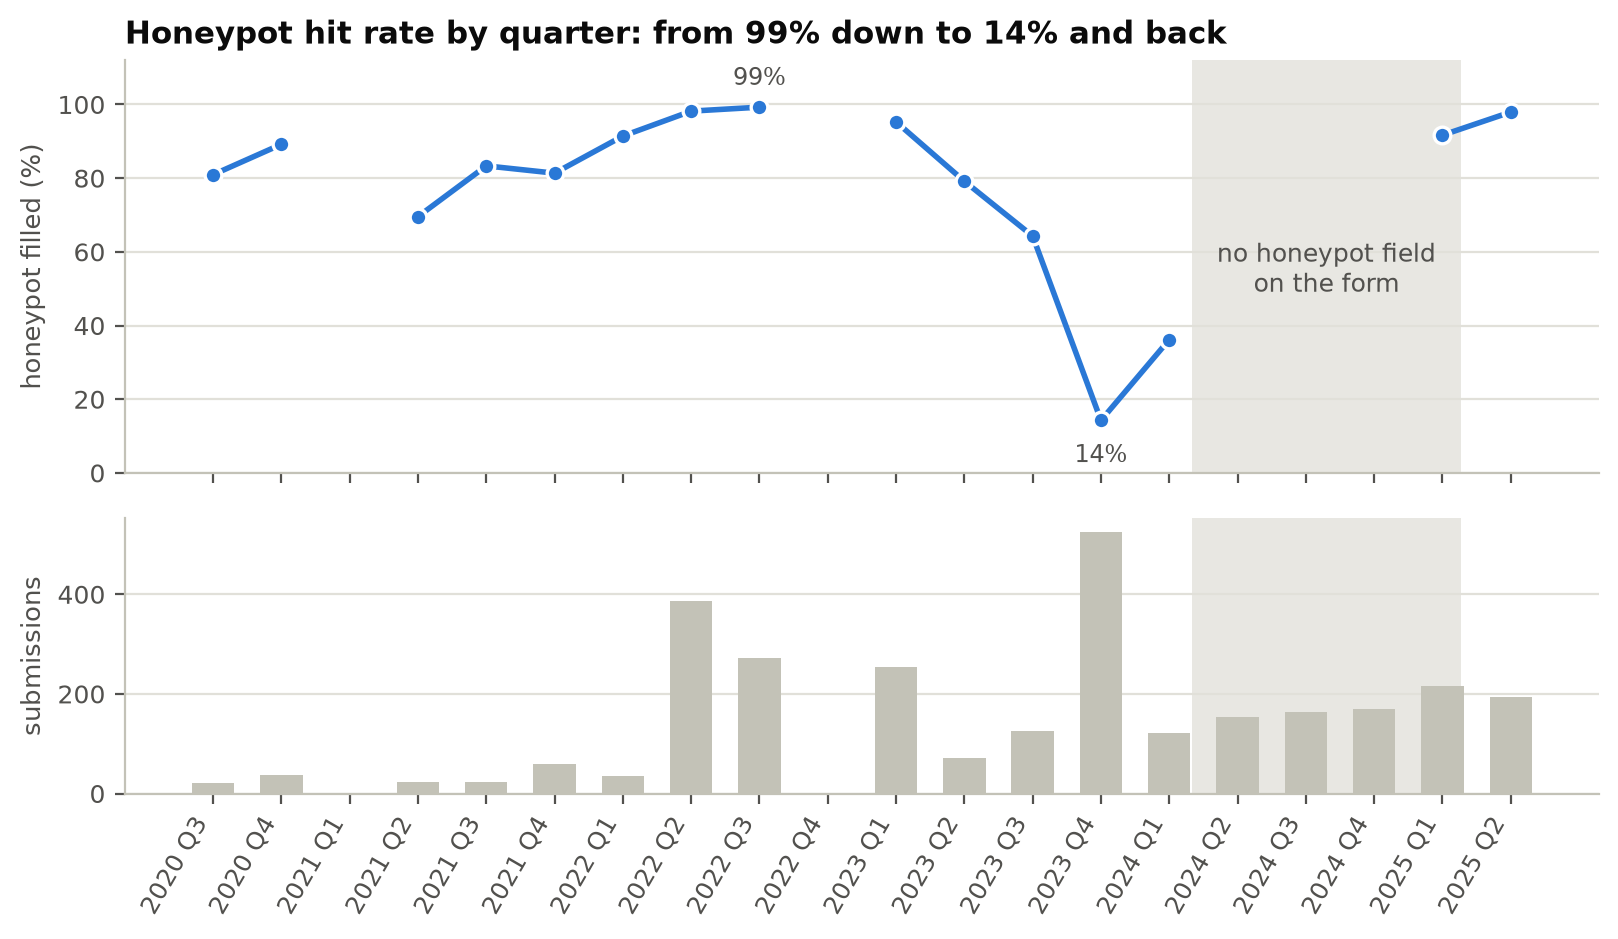
\includegraphics[width=\columnwidth]{fig_honeypot_rate.png}}
\caption{Honeypot hit rate and number of submissions per quarter. The shaded band is the window in which the
form had no honeypot field. Empty quarters are missing from the export.}
\label{fig:rate}
\end{figure}

\subsection{Association rules}

Apriori finds 281 frequent itemsets and 1,183 rules. Table~\ref{tab:rules} lists the strongest rules that end
in a honeypot outcome. The rows matching the first group are one campaign, the ``financial robot'' adverts: a
medium-length message about money with one link. The rows matching the second group are a single sentence,
``Hi, I wanted to know your price'', machine-translated into dozens of languages and sent under joined names.
That sender completes name, e-mail, phone and message and skips the hidden field. Lowering the support
threshold to 0.05 raises the number of itemsets to 399 and raising it to 0.30 cuts it to 85; the chosen values
keep every rule above a tenth of the submissions.

\begin{table}[t]
\caption{Strongest Association Rules Ending in a Honeypot Outcome}
\label{tab:rules}
\centering
\begin{tabular}{@{}p{4.4cm}ccc@{}}
\toprule
\textbf{Antecedent} & \textbf{Supp.} & \textbf{Conf.} & \textbf{Lift} \\
\midrule
\multicolumn{4}{@{}l}{\emph{Consequent: honeypot filled (base rate 0.71)}} \\
medium length, money topic & 0.34 & 0.96 & 1.35 \\
one URL, money topic & 0.35 & 0.92 & 1.29 \\
medium length & 0.50 & 0.92 & 1.29 \\
\midrule
\multicolumn{4}{@{}l}{\emph{Consequent: honeypot empty (base rate 0.29)}} \\
short, joined name & 0.14 & 0.88 & 3.05 \\
no URL, joined name & 0.15 & 0.86 & 3.00 \\
short, free e-mail & 0.14 & 0.86 & 2.98 \\
\bottomrule
\end{tabular}
\end{table}

\subsection{Campaigns}

Cosine similarity already shows the campaign structure: 51\% of the templates have another template at
similarity 0.5 or more and 16\% at 0.9 or more. K-means gives no sharp elbow, and the silhouette rises slowly
from 0.18 at $k=4$ to 0.26 at $k=16$, the value used. A silhouette of this size means coarse topics, not crisp
groups. The clusters are nevertheless readable from their top terms (Fig.~\ref{fig:campaigns}): financial
adverts, backlink and SEO offers, pharmacy, casino, crypto wallets and several Russian-language groups. A
further 139 templates share no vocabulary with any other template and form their own group; most are one-line
messages, among them the multilingual price enquiry, which no text clustering can assemble because its
versions share no words. Apriori caught that campaign through its shape. The two methods complement each other.

Honeypot hit rates range from 0\% to 100\% across campaigns. The largest campaign, the financial adverts with
854 submissions, is caught 98\% of the time; the no-shared-vocabulary group, 446 submissions, 24\% of the time.
The swings of Fig.~\ref{fig:rate} follow from the campaign mix.

K-medoids gives each cluster a real message as its centre. On the same sample its silhouette is 0.21 against
0.26 for K-means, and the two partitions agree only partly (adjusted Rand index 0.36). EM in one dimension
separates one-line messages (typical length 83 characters, weight 0.65) from full adverts (750 characters). On
the text representation 14\% of the templates have no component with a membership above 0.9, and BIC keeps
falling as components are added. All three methods say the same thing: the structure is real but not sharp.

\begin{figure*}[t]
\centerline{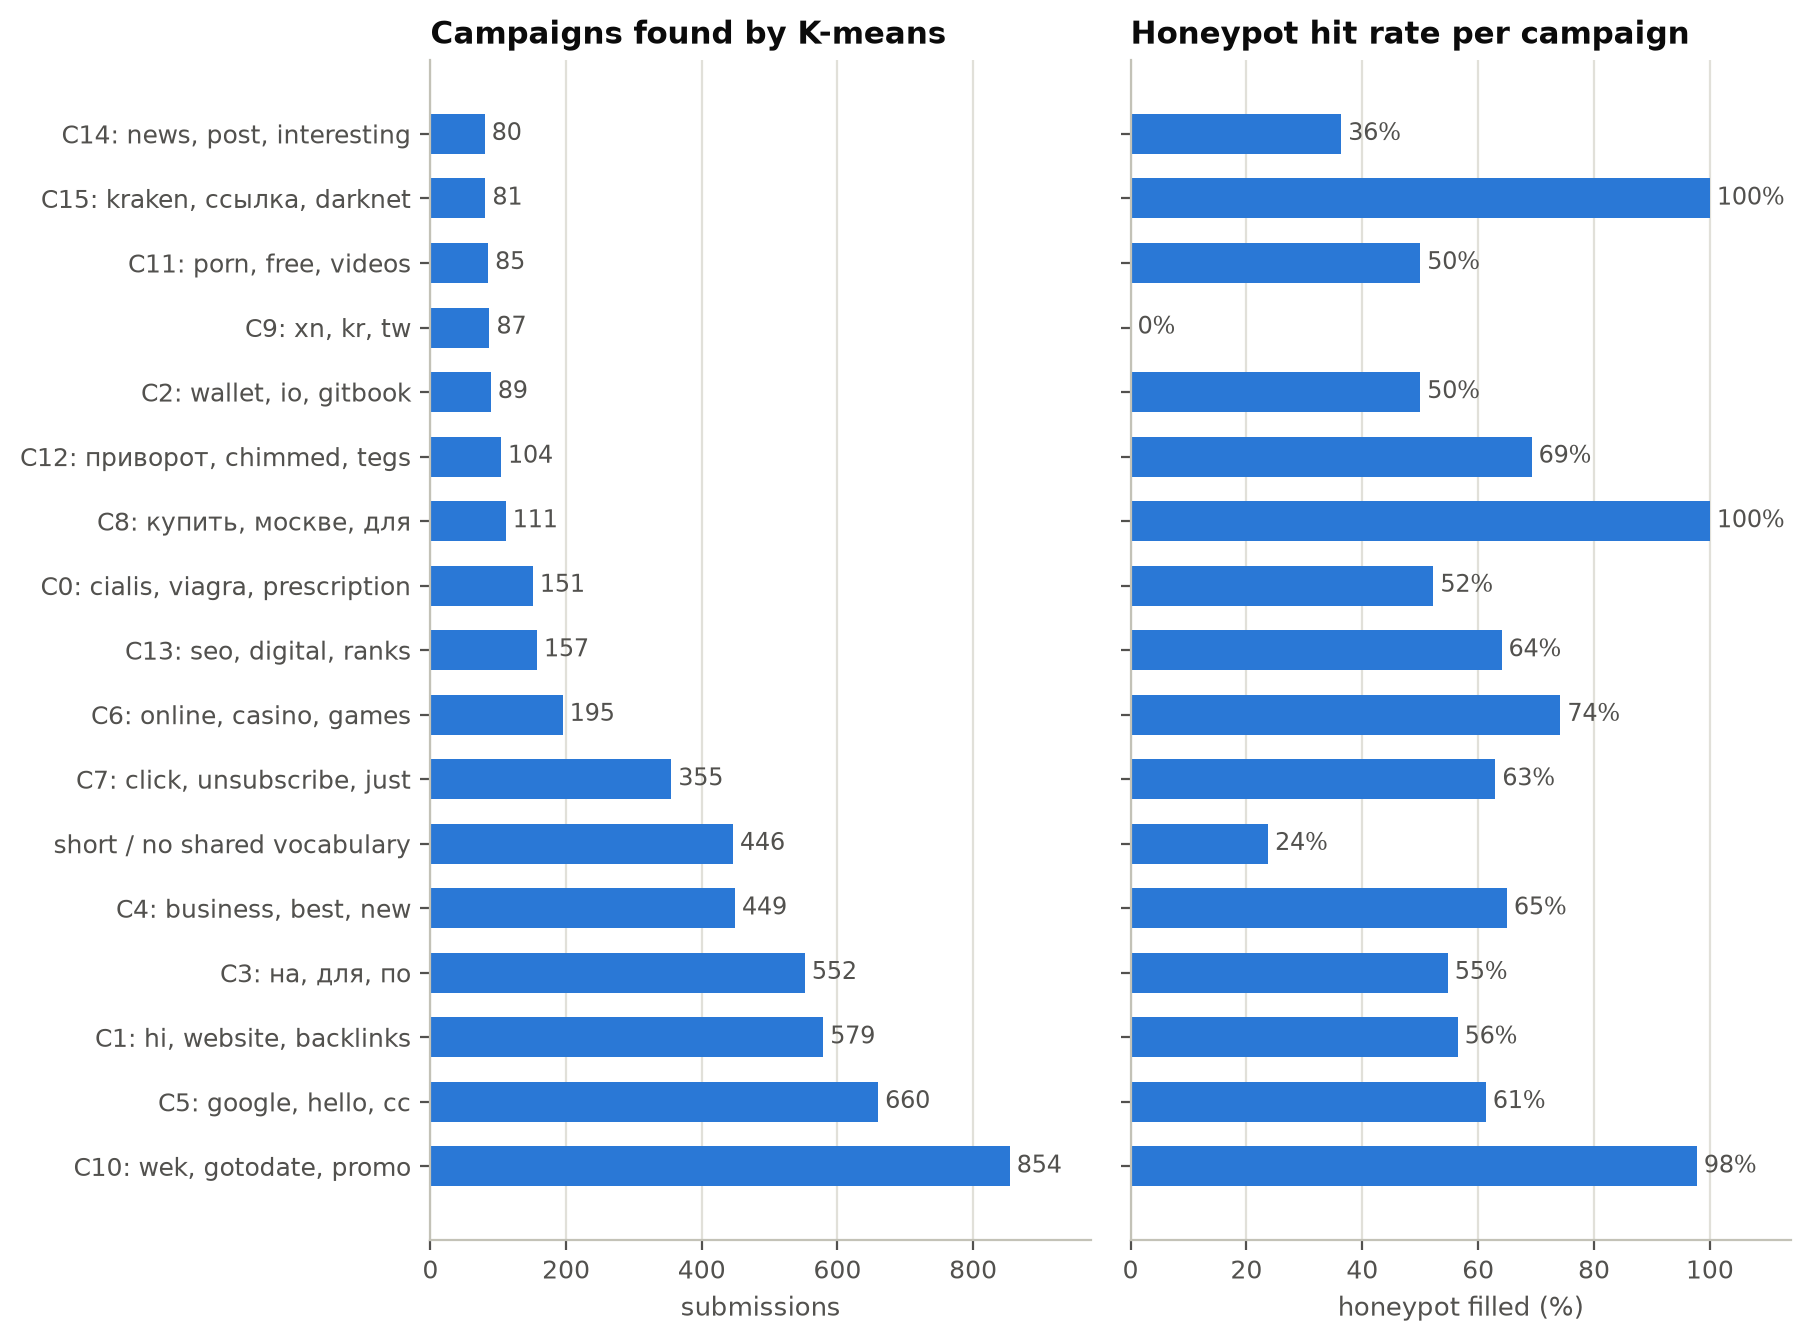
\includegraphics[width=0.82\textwidth]{fig_campaigns.png}}
\caption{Campaigns found by K-means ($k=16$), named by their most characteristic terms, with the number of
submissions and the honeypot hit rate of each.}
\label{fig:campaigns}
\end{figure*}

\subsection{Task A: predicting honeypot evasion}

\textbf{Split criteria.} At the root node the entropy is 0.866 bits. Table~\ref{tab:split} shows why
information gain alone is not enough. The template identifier has the highest gain because it splits the data
into hundreds of tiny pure groups, which would predict nothing for a new template. Its split information is
equally large, so its gain ratio is low and C4.5 chooses a real attribute, the joined-name flag.

\begin{table}[t]
\caption{Root Split: Information Gain (ID3) Against Gain Ratio (C4.5)}
\label{tab:split}
\centering
\begin{tabular}{@{}lccc@{}}
\toprule
\textbf{Attribute} & \textbf{Values} & \textbf{Gain} & \textbf{Gain ratio} \\
\midrule
Template id & 824 & \textbf{0.642} & 0.072 \\
Length bin & 5 & 0.265 & 0.163 \\
URL bin & 3 & 0.212 & 0.159 \\
Name is joined & 2 & 0.201 & \textbf{0.249} \\
E-mail domain & 40 & 0.149 & 0.046 \\
Money keyword & 2 & 0.106 & 0.107 \\
\bottomrule
\end{tabular}
\end{table}

\textbf{Model comparison.} Table~\ref{tab:taska} and Fig.~\ref{fig:taska} give the results. In
cross-validation the learned models reach a balanced accuracy of 0.73 to 0.79 and an AUC of up to 0.88. No
score is near 1.00, which is what an observed, noisy label looks like. A one-line rule, ``the message has a
URL'', already reaches 0.76; the learned models are better at ranking (AUC 0.80 to 0.88 against 0.76).

On the later period only logistic regression keeps a useful score, 0.69 with an AUC of 0.77. The other learned
models fall to between 0.49 and 0.57, below the URL rule. The test period is small, 372 submissions of which 71
have an empty honeypot, so differences of a few points carry no weight; the gaps reported here are far larger.
The cause is concept drift \cite{gama2014}. In 2025 almost every submission fills the field, including the
one-line enquiry that almost never did in 2023, and the form itself changed at that time
(Section~\ref{sec:window}). Honeypot behaviour depends on the bot and on how the form presents the field.
Content features see neither.

Other observations follow the theory. Bernoulli Naive Bayes on the binary flags (0.78) beats Gaussian Naive
Bayes on all features (0.63), because count features are far from Gaussian. Scaling raises KNN from 0.75 to
0.78, and KNN stores the whole training set (662~KB against about 2.5~KB for the linear models). The
Mahalanobis classifier beats a Euclidean nearest-mean classifier on the same principal components, 0.785
against 0.767. The perceptron matches logistic regression in balanced accuracy but has the lowest AUC (0.80):
it outputs a decision, not a graded score, and its error count never reaches zero because the classes are not
linearly separable. The tuned tree (depth 4) is the least stable model; its first split is the joined-name
flag, the attribute chosen by gain ratio and found by Apriori. The MLP shows where extra capacity goes: it
reaches 0.89 on the rows it was trained on and 0.51 on the later period, against 0.82 and 0.69 for logistic
regression. PCA leaves KNN unchanged (0.783 against 0.786) and costs logistic regression 2.5 points, so it is
applied only where it is required.

\textbf{Effect of the label audit.} Had the recorded label been trusted, the test period would have had 1,019
rows instead of 372, 30\% ``filled'' instead of 81\%, and most models would have scored 5 to 14 points higher,
because the window adds hundreds of rows labelled ``empty'' that the models happen to call ``empty''. The
conclusions would have rested on rows whose label says nothing about the sender.

\begin{table}[t]
\caption{Task A: Balanced Accuracy and AUC, Grouped Cross-Validation and Time Split}
\label{tab:taska}
\centering
\begin{tabular}{@{}lcccc@{}}
\toprule
 & \multicolumn{2}{c}{\textbf{5-fold CV}} & \multicolumn{2}{c}{\textbf{2024--2025}} \\
\textbf{Model} & \textbf{Bal.} & \textbf{AUC} & \textbf{Bal.} & \textbf{AUC} \\
\midrule
Majority class & 0.500 & 0.500 & 0.500 & 0.500 \\
Rule ``has a URL'' & 0.756 & 0.756 & 0.609 & 0.609 \\
\midrule
Naive Bayes (Bernoulli) & 0.779 & 0.857 & 0.492 & 0.472 \\
Logistic regression & \textbf{0.791} & \textbf{0.880} & \textbf{0.689} & \textbf{0.765} \\
Decision tree & 0.734 & 0.826 & 0.539 & 0.628 \\
KNN ($k=7$) & 0.783 & 0.868 & 0.570 & 0.557 \\
Mahalanobis (PCA) & 0.785 & 0.866 & 0.506 & 0.529 \\
Perceptron & 0.789 & 0.796 & 0.560 & 0.570 \\
MLP, one hidden layer & 0.775 & 0.841 & 0.513 & 0.587 \\
\bottomrule
\end{tabular}
\end{table}

\begin{figure}[t]
\centerline{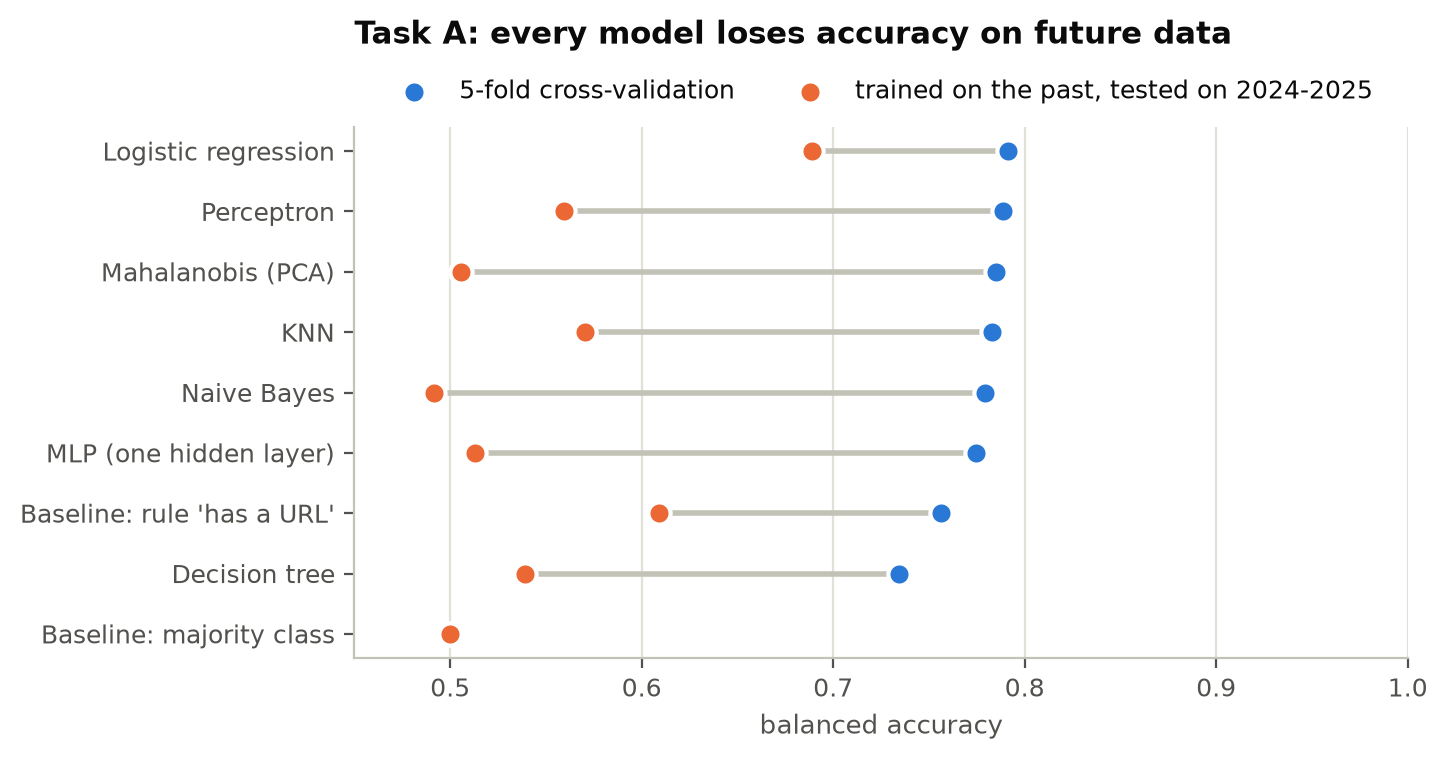
\includegraphics[width=\columnwidth]{fig_task_a_models.png}}
\caption{Task A: balanced accuracy in grouped cross-validation and on the later period.}
\label{fig:taska}
\end{figure}

\subsection{Task B: spam versus legitimate}

Table~\ref{tab:taskb} gives the results. In cross-validation every word-based model reaches a balanced
accuracy of 0.95 to 0.97. On these numbers the task looks solved.

Much of that score is the source difference. Message length alone, with no words, reaches 0.79. The tokens
that most indicate spam are URL fragments and Cyrillic words, and the tokens that most indicate a legitimate
message are SMS slang. The checks separate what is real from what is not (Fig.~\ref{fig:controls}). Restricting
both classes to 20--200 characters pushes the length baseline to 0.54, close to chance, while the word models
stay at 0.94 or above, so words carry signal beyond length. On the same-source test the models still rank SMS
spam above legitimate SMS (AUC 0.69 to 0.92, except the tree at 0.46), yet at the default threshold logistic
regression catches only 22\% of the SMS spam. The models know form spam, and that knowledge transfers only
partly to another kind of spam.

The fourth check reverses the ranking. The perceptron and the MLP lead the cross-validation table and flag 6
and 7 of the 40 genuine contact-form messages. Naive Bayes, logistic regression and the tree flag one. The
extra in-distribution accuracy came from fitting the two collections more tightly.

The errors of the chosen model are instructive. In cross-validation it passes 215 of the 3,122 spam templates.
Those have a median length of 23 characters against 354 for the templates it catches, and 11\% of them contain a
URL against 92\%. They are bare names, random strings and the one-line multilingual enquiry: the senders that
also evade the honeypot. The two defences share a blind spot, and what identifies these senders is their
shape, which the association rules capture.

For Naive Bayes, 13,463 of the 17,195 vocabulary words never occur in the legitimate class, so without
smoothing almost every spam word would force a zero probability. Laplace smoothing with $\alpha = 1$ removes
the problem but is not the best value here: $\alpha = 0.01$ raises balanced accuracy from 0.949 to 0.964,
because one added count for each of 17,195 words is large against the 44,365 words of the legitimate class.

\textbf{Model selection.} The software needs a probability, a model under 5~MB and a prediction under 10~ms.
We had fixed in advance that the candidate with the best cross-validated F1 would be chosen. That rule does not
discriminate: four candidates lie within 0.01 F1 of the best. Among those four we therefore chose the model
that flags the fewest genuine messages, with same-source AUC as the tie-break. This selects \textbf{logistic
regression} (821~KB, under 1~ms per message). The 40-message set was thus used for selection, and its count
for the chosen model is no longer an untouched estimate. At a threshold of 0.7 the model flags none of the 40
genuine messages and recalls 87\% of form spam.

\begin{table}[t]
\caption{Task B: Cross-Validation and Out-of-Corpus Checks}
\label{tab:taskb}
\centering
\begin{tabular}{@{}l@{\hspace{5pt}}c@{\hspace{5pt}}c@{\hspace{5pt}}c@{\hspace{5pt}}c@{\hspace{5pt}}c@{}}
\toprule
 & \multicolumn{3}{c}{\textbf{5-fold CV}} & \textbf{Same-} & \textbf{Genuine} \\
\textbf{Model} & \textbf{Bal.} & \textbf{F1} & \textbf{AUC} & \textbf{source AUC} & \textbf{flagged/40} \\
\midrule
Length only & 0.790 & 0.746 & 0.871 & -- & -- \\
\midrule
Naive Bayes & 0.949 & 0.945 & 0.977 & 0.768 & 1 \\
Logistic regression & 0.964 & 0.963 & \textbf{0.996} & 0.912 & 1 \\
Decision tree & 0.961 & 0.958 & 0.980 & 0.464 & 1 \\
KNN, cosine & 0.966 & 0.964 & 0.994 & 0.690 & 3 \\
Mahalanobis (LSA) & 0.957 & 0.953 & 0.994 & 0.873 & \textbf{0} \\
Perceptron & \textbf{0.973} & \textbf{0.967} & 0.994 & 0.828 & 6 \\
MLP, one hidden layer & 0.969 & 0.965 & 0.995 & \textbf{0.920} & 7 \\
\bottomrule
\end{tabular}
\end{table}

\begin{figure}[t]
\centerline{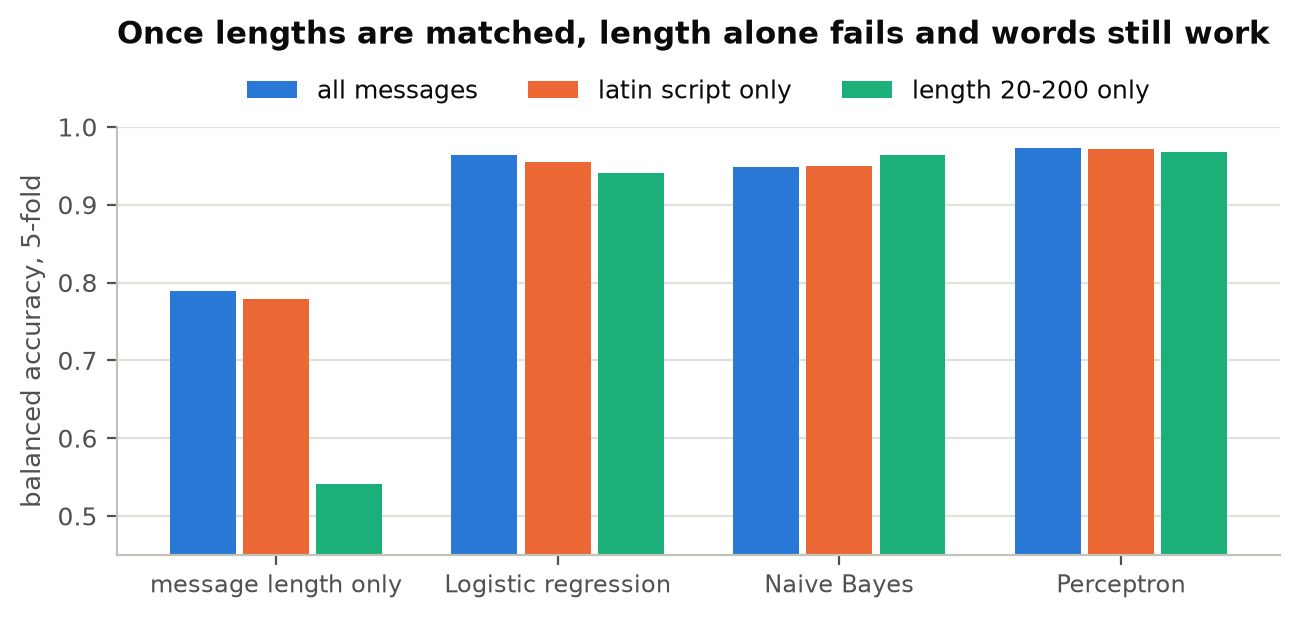
\includegraphics[width=\columnwidth]{fig_task_b_controls.png}}
\caption{Task B: balanced accuracy on all messages, on Latin-script messages only, and on messages of 20--200
characters. Matching lengths removes the advantage of the length baseline and leaves the word models intact.}
\label{fig:controls}
\end{figure}

\subsection{Which algorithm suits which task}

Scoring well on data drawn like the training data says little about holding up when the data differs. The
perceptron and the MLP lead Task B in cross-validation and flag the most genuine messages. Most models that
look acceptable in Task A cross-validation are at chance a year later. Logistic regression is at or near the
top in-distribution in both tasks and is the most reliable outside it. Naive Bayes is a sound fallback when no
tuning is possible. The decision tree is valuable for explanation and poor for scoring. KNN is unsuitable for a
small server. The Mahalanobis classifier demonstrates the value of the covariance correction but needs PCA to
be computable. With a few thousand rows and a moving target, a simple probabilistic model is the right choice.

\section{System Integration}

The form's software is a PHP and MySQL application that scores each submission with weighted rules and blocks
it at a total of 100. We added a small Python service that loads the exported model. For each submission the
service masks e-mail addresses and phone numbers exactly as the training data was masked and returns the spam
probability, the words that raised it, the nearest campaign centroid, and the mined association rules whose
conditions hold, which cover the short messages the text model cannot read. A new rule adds a weight of 60 when the probability reaches the threshold. The model alone
therefore marks a submission as high risk and does not block it; blocking needs a second signal. We chose this
because the model was trained without real legitimate contact-form traffic. If the service is unreachable the
rule does not trigger and the other rules continue to work.

A dashboard page shows the model comparison, the campaigns, the mined rules beside the hand-written ones, and
an OLAP view that offers roll-up, drill-down, slice and dice through SQL \texttt{GROUP BY} with
\texttt{ROLLUP}. Loading the 2,741 timestamped submissions with a message into the system and scoring each
took 113 seconds, about 41~ms per submission including the HTTP call and the database writes.

\section{Limitations}

The data come from one site and contain no genuine enquiries. The legitimate class of Task B is SMS, and the 40
contact-form messages are written by us; the scores describe this corpus and the model must be retrained on
the operator's own legitimate traffic. The window without a honeypot was found in the data before it was confirmed, and the
older export, which has no timestamps, cannot be checked in the same way. The Task A test period is small. Only exact templates were de-duplicated for Task B, so
near-duplicates can fall on both sides of a fold and make its cross-validation scores optimistic. Association
rules report co-occurrence in the period they were mined from, and Task A shows one of them reversing later.

\section{Conclusion}

A honeypot field caught 98\% of the submissions to this form in one year and 14\% in one quarter of the next.
Its hit rate follows the campaign mix, and for a year the signal was missing altogether, which only a check of
the label revealed. Whether a sender fills the field is moderately predictable inside a period (balanced
accuracy 0.79) and poorly predictable forward in time (0.69 for the best model). For filtering by content,
headline accuracy is a poor guide: seven models score alike in cross-validation, and out-of-corpus checks
separate them. The practical result is a small logistic regression model, used as one signal among several,
and a view of the traffic as campaigns. Future work is to collect genuine submissions for retraining, to
retrain on a schedule to follow drift, and to add features of message shape to both the clustering and the
classifier, so that short multilingual campaigns are grouped and caught.

\begin{thebibliography}{00}
\bibitem{imperva2025} Imperva, ``2025 Bad Bot Report,'' Thales, Tech. Rep., Apr. 2025.
\bibitem{vonahn2003} L. von Ahn, M. Blum, N. J. Hopper, and J. Langford, ``CAPTCHA: Using hard AI problems for security,'' in \emph{Advances in Cryptology -- EUROCRYPT 2003}, LNCS vol. 2656. Springer, 2003, pp. 294--311.
\bibitem{spitzner2002} L. Spitzner, \emph{Honeypots: Tracking Hackers}. Boston, MA, USA: Addison-Wesley, 2002.
\bibitem{geerling2011} J. Geerling, ``Introducing the Honeypot form spam protection module for Drupal,'' 2011. [Online]. Available: \url{https://www.jeffgeerling.com/blog/2011/introducing-honeypot-form-spam/}
\bibitem{prince2005} M. B. Prince, B. M. Dahl, L. Holloway, A. M. Keller, and E. Langheinrich, ``Understanding how spammers steal your e-mail address: An analysis of the first six months of data from Project Honey Pot,'' in \emph{Proc. 2nd Conf. Email and Anti-Spam (CEAS)}, 2005.
\bibitem{sahami1998} M. Sahami, S. Dumais, D. Heckerman, and E. Horvitz, ``A Bayesian approach to filtering junk e-mail,'' in \emph{Learning for Text Categorization: Papers from the 1998 Workshop}, AAAI Tech. Rep. WS-98-05, 1998.
\bibitem{metsis2006} V. Metsis, I. Androutsopoulos, and G. Paliouras, ``Spam filtering with naive Bayes -- which naive Bayes?'' in \emph{Proc. 3rd Conf. Email and Anti-Spam (CEAS)}, 2006.
\bibitem{almeida2011} T. A. Almeida, J. M. G. Hidalgo, and A. Yamakami, ``Contributions to the study of SMS spam filtering: New collection and results,'' in \emph{Proc. 11th ACM Symp. Document Engineering (DocEng)}, 2011, pp. 259--262.
\bibitem{salton1988} G. Salton and C. Buckley, ``Term-weighting approaches in automatic text retrieval,'' \emph{Inf. Process. Manag.}, vol. 24, no. 5, pp. 513--523, 1988.
\bibitem{deerwester1990} S. Deerwester, S. T. Dumais, G. W. Furnas, T. K. Landauer, and R. Harshman, ``Indexing by latent semantic analysis,'' \emph{J. Amer. Soc. Inf. Sci.}, vol. 41, no. 6, pp. 391--407, 1990.
\bibitem{kreibich2009} C. Kreibich, C. Kanich, K. Levchenko, B. Enright, G. M. Voelker, V. Paxson, and S. Savage, ``Spamcraft: An inside look at spam campaign orchestration,'' in \emph{Proc. 2nd USENIX Workshop Large-Scale Exploits and Emergent Threats (LEET)}, 2009.
\bibitem{kaufman2012} S. Kaufman, S. Rosset, C. Perlich, and O. Stitelman, ``Leakage in data mining: Formulation, detection, and avoidance,'' \emph{ACM Trans. Knowl. Discov. Data}, vol. 6, no. 4, art. 15, 2012.
\bibitem{geirhos2020} R. Geirhos, J.-H. Jacobsen, C. Michaelis, R. Zemel, W. Brendel, M. Bethge, and F. A. Wichmann, ``Shortcut learning in deep neural networks,'' \emph{Nature Mach. Intell.}, vol. 2, no. 11, pp. 665--673, 2020.
\bibitem{gama2014} J. Gama, I. \v{Z}liobait\.{e}, A. Bifet, M. Pechenizkiy, and A. Bouchachia, ``A survey on concept drift adaptation,'' \emph{ACM Comput. Surv.}, vol. 46, no. 4, art. 44, 2014.
\bibitem{chaudhuri1997} S. Chaudhuri and U. Dayal, ``An overview of data warehousing and OLAP technology,'' \emph{ACM SIGMOD Rec.}, vol. 26, no. 1, pp. 65--74, 1997.
\bibitem{agrawal1994} R. Agrawal and R. Srikant, ``Fast algorithms for mining association rules,'' in \emph{Proc. 20th Int. Conf. Very Large Data Bases (VLDB)}, 1994, pp. 487--499.
\bibitem{jolliffe2002} I. T. Jolliffe, \emph{Principal Component Analysis}, 2nd ed. New York, NY, USA: Springer, 2002.
\bibitem{macqueen1967} J. MacQueen, ``Some methods for classification and analysis of multivariate observations,'' in \emph{Proc. 5th Berkeley Symp. Math. Statist. Probab.}, vol. 1, 1967, pp. 281--297.
\bibitem{kaufman1990} L. Kaufman and P. J. Rousseeuw, \emph{Finding Groups in Data: An Introduction to Cluster Analysis}. New York, NY, USA: Wiley, 1990.
\bibitem{dempster1977} A. P. Dempster, N. M. Laird, and D. B. Rubin, ``Maximum likelihood from incomplete data via the EM algorithm,'' \emph{J. Roy. Statist. Soc. B}, vol. 39, no. 1, pp. 1--38, 1977.
\bibitem{rousseeuw1987} P. J. Rousseeuw, ``Silhouettes: A graphical aid to the interpretation and validation of cluster analysis,'' \emph{J. Comput. Appl. Math.}, vol. 20, pp. 53--65, 1987.
\bibitem{quinlan1986} J. R. Quinlan, ``Induction of decision trees,'' \emph{Mach. Learn.}, vol. 1, no. 1, pp. 81--106, 1986.
\bibitem{quinlan1993} J. R. Quinlan, \emph{C4.5: Programs for Machine Learning}. San Mateo, CA, USA: Morgan Kaufmann, 1993.
\bibitem{cover1967} T. M. Cover and P. E. Hart, ``Nearest neighbor pattern classification,'' \emph{IEEE Trans. Inf. Theory}, vol. 13, no. 1, pp. 21--27, 1967.
\bibitem{mahalanobis1936} P. C. Mahalanobis, ``On the generalised distance in statistics,'' \emph{Proc. Nat. Inst. Sci. India}, vol. 2, no. 1, pp. 49--55, 1936.
\bibitem{rosenblatt1958} F. Rosenblatt, ``The perceptron: A probabilistic model for information storage and organization in the brain,'' \emph{Psychol. Rev.}, vol. 65, no. 6, pp. 386--408, 1958.
\bibitem{pedregosa2011} F. Pedregosa \emph{et al.}, ``Scikit-learn: Machine learning in Python,'' \emph{J. Mach. Learn. Res.}, vol. 12, pp. 2825--2830, 2011.
\end{thebibliography}

\end{document}
